\hypertarget{preface}{%
\section{Preface}\label{preface}}

\hypertarget{uxfcber-tvd-criticalpatchreport}{%
\subsection{Über
TVD-CriticalPatchReport}\label{uxfcber-tvd-criticalpatchreport}}

Das Oracle Critical Patch Advisory wird alle drei Monate veröffentlicht
und behebt Sicherheitsprobleme in Oracle-Datenbanken, Applikationsserver
und anderen Oracle Produkten. In vielen Fällen ist es schwierig zu
entscheiden, ob ein kritischer Patch sofort in einer Produktionsumgebung
angewendet werden muss oder nicht. Hier kommt der Trivadis Critical
Patch Report ins Spiel. Trivadis testet mehrere kritische Patches auf
verschiedenen Oracle-Produkten und -Versionen. Insbesondere die
kritischen Patch-Updates für die Oracle Datenbanken auf den Plattformen
SUN, AIX, Linux und Windows sowie den Oracle Applikation Server, der
unter Linux und Windows getestet wird. Die Testergebnisse werden im
TVD-CriticalPatchReport zusammengefasst und im gleichen Zyklus
freigegeben. Der Bericht hilft bei der Entscheidung, ob ein kritisches
Patch-Update installiert werden muss oder nicht, ausserdem gibt er Ihnen
wertvolle Tipps.

Ihre Vorteile

\begin{itemize}
\tightlist
\item
  Empfehlungen: Wann Sie den Patch installieren sollen - und wann nicht.
\item
  Tipps, die Sie bei der Installation der CPU beachten sollten.
\item
  Informationen darüber, ob sich die Datenbank nach der Installation der
  CPU anders verhält.
\end{itemize}

Der TVD-CriticalPatchReport wird im Rahmen des Managed Service Agreement
an Trivadis Kunden verteilt oder kann alternativ als separater
Service\footnote{\href{https://www.trivadis.com/en/trivadis-toolbox}{Trivadis
  Toolbox} and
  \href{https://www.trivadis.com/en/trivadis-toolbox\#cpr}{TVD-CriticalPatchReport}}
erworben werden.

\hypertarget{copyright-und-lizenz}{%
\subsection{Copyright und Lizenz}\label{copyright-und-lizenz}}

Copyright© 2019 Trivadis AG. Dieses Dokument wird sowohl als dedizierter
Service als auch als Teil des Managed Service Agreement den Trivadis
Kunden zur Verfügung gestellt. Alle Rechte vorbehalten. Nachdruck und
Vervielfältigung, einschliesslich Speicherung und Verwendung auf
optischen und elektronischen Medien, bedarf der Zustimmung der Trivadis
AG.

Die Qualifikationen der Oracle Critical Patch Updates (CPU) basieren auf
Oracle-Standardinstallationen. Die technischen Spezialisten von Trivadis
führen die Tests und Bewertungen durch. Es kann jedoch nicht
ausgeschlossen werden, dass Systeme in einer Kundenumgebung nach dem
Anwenden bzw. Nicht-anwenden der CPUs nicht wie erwartet funktionieren.
Für Schäden, die durch die Verwendung bzw. Nichtverwendung von CPUs
entstehen, übernimmt Trivadis keine Haftung.

Oracle und Java sind eingetragene Marken von Oracle und/oder seinen
verbundenen Unternehmen. Andere Namen können Marken ihrer jeweiligen
Eigentümer sein. Für die in diesem Bericht aufgeführten Oracle-Produkte
gelten die Lizenzbedingungen von Oracle.

\hypertarget{dokumentinformation}{%
\subsection{Dokumentinformation}\label{dokumentinformation}}

\begin{itemize}
\tightlist
\item
  \textbf{Document:} Trivadis CPU-Report
\item
  \textbf{Classification:} Restricted / Trivadis customer
\item
  \textbf{Status:} Published
\item
  \textbf{Last changes:} 2019.10.16
\item
  \textbf{Document name:} Example\_documentation.pdf
\end{itemize}

\begin{longtable}[]{@{}ll@{}}
\toprule
Hauptautoren & Mitwirkende \& Reviewer\tabularnewline
\midrule
\endhead
Stefan Oehrli & Patrick Joss\tabularnewline
\bottomrule
\end{longtable}

\hypertarget{revisionshistorie}{%
\subsection{Revisionshistorie}\label{revisionshistorie}}

\begin{longtable}[]{@{}llll@{}}
\toprule
Version & Datum & Visum & Bemerkung\tabularnewline
\midrule
\endhead
0.1 & 2019.10.16 & soe & Intial Release CPU Report July
2019\tabularnewline
0.2 & 2019.07.20 & & Add Database check information\tabularnewline
0.3 - 0.8 & & & Complete revision of the CPU Report
template\tabularnewline
1.0 & & & Finalize CPU Report July 2019\tabularnewline
\bottomrule
\end{longtable}

Bei Fragen stehen wir Ihnen gerne via \url{cpureport@trivadis.com} zur
Verfügung.

\hypertarget{generelle-information}{%
\section{Generelle Information}\label{generelle-information}}

\hypertarget{datenbank-versionen}{%
\subsection{Datenbank Versionen}\label{datenbank-versionen}}

Mit dem neuen Release Zyklus hat Oracle eine neue Bezeichnung für die
Critical Patch Updates eingeführt. Die Critical Patch Updates für Oracle
12.2.0.1 heissen Release-Updates, abgekürzt RU. Dementsprechend wurden
unsere Tests angepasst. Bei Oracle 12c werden neu die Patch Set Updates
respektive Release Updates, wo verfügbar, getestet. Aktuell gibt es nur
Patch Set Updates für 12.1.0.2, respektive Release Updates für Oracle
12.2.0.1, 18.0.0.0 und 19.0.0.0. Für Oracle 11.2.0.4 gibt es seit Januar
2019 keinen regulären Critical Patch Update mehr. Der Premier Support
endete per 1. Januar 2015. Per 31. Dezember 2018 ist auch der Extended
Support Fee Waiver abgelaufen. Seit dem 1. Januar 2019 wird für diesen
Release ein Extended Support Vertrag benötigt, um Patch sowie Critical
Patch Update herunterladen zu können. Siehe auch My Oracle Support
742060.1 Note Release Schedule of Current Database Releases. Siehe auch
in der My Oracle Support
\href{https://support.oracle.com/epmos/faces/DocumentDisplay?id=742060.1}{742060.1}
\emph{Note Release Schedule of Current Database Releases}.

Neben einem PSU respektive RU für die Datenbank, gibt es für Oracle Java
VM entsprechende Patches. Mehr dazu in der My Oracle Support Note
\href{https://support.oracle.com/epmos/faces/DocumentDisplay?id=1929745.1}{1929745.1}
In der Note wird darauf hingewiesen, dass die Post Install Tasks im
UPGRADE Mode ausgeführt werden sollten, wenn die JavaVM installiert ist.

Neben dem PSU, Oracle Java VM PSU gibt es zusätzlich quartalweise ein
proaktiver Bundle Patch. Die Bundle Patches sind ein Superset der PSU
und enthalten neben den Security Fixes weiter Bugfixes. Mehr dazu in der
My Oracle Support Note
\href{https://support.oracle.com/epmos/faces/DocumentDisplay?id=1998563.1}{1998563.1}
und
\href{https://support.oracle.com/epmos/faces/DocumentDisplay?id=1962125.1}{1962125.1}.
Mit der Installation des Combo Patch, welcher den PSU, JVM PSU und BP
enthält, ist das Datenbank System jeweils auf dem aktuellsten
Patchlevel.

Seit November 2015 hat Oracle für die Versionsbezeichnung der neuen
Bundle Patches, Patch Set Updates und Security Patches ein neues Format
eingeführt. Neu wird statt der 5. Stelle das Release Datum in der Form
YYMMDD angehängt:

\begin{itemize}
\tightlist
\item
  \textbf{YY} letzte zwei Ziffern vom Jahr
\item
  \textbf{MM} Monat (2 Ziffern)
\item
  \textbf{DD} Tag im Monat (2 Ziffern)
\end{itemize}

\hypertarget{weblogic-server}{%
\subsection{Weblogic Server}\label{weblogic-server}}

Bis zur Weblogic Version 12.1.1 wurden die Patches jeweils mit BEA Smart
Update (BSU) eingespielt. Ab Version 12.1.2 wird Smart Update durch das
im Datenbankumfeld bekannte OPatch abgelöst. Ein Patchen mit BSU ist ab
dieser Version nicht mehr möglich.

\hypertarget{trivadis-empfehlung}{%
\section{Trivadis Empfehlung}\label{trivadis-empfehlung}}

\hypertarget{oracle-datenbank}{%
\subsection{Oracle Datenbank}\label{oracle-datenbank}}

Das höchste Base Ranking im Rahmen des Common Vulnerability Scoring
System (\href{http://www.first.org/cvss/}{CVSS}) im Bereich der reinen
Datenbank liegt beim vorliegenden CPU bei 9.8 von 10 und betrifft die
Core RDBMS Komponente in 11.2.0.4, 12.1.0.2, 12.2.0.1, 18c und 19c auf
allen Betriebssystemen. Zudem kann diese Sicherheitslücke remote über
das Netzwerk ausgenutzt werden.

Mit 9 Korrekturen für Sicherheitslücken beim Oracle Database Server ist
dies ein etwas grösserer CPU. Die Sicherheitslücken können teilweise
remote über das Netzwerk ausgenutzt werden.

Der CPU konnte auf allen unseren Testumgebungen mit kleineren Issues
installiert werden. Aufgrund des sehr hohen CVSS Rating für Core RDBMS
wird empfohlen das Critical Patch Update auf allen entsprechenden
Systemen einzuspielen. Bei allen Systemen ist es ebenfalls sinnvoll, das
Critical Patch Update einzu-spielen, speziell wenn das letzte Critical
Patch Update übersprungen wurde. Die My Oracle Support Note
\href{https://support.oracle.com/epmos/faces/DocumentDisplay?id=1929745.1}{1929745.1}
enthält weitere Informationen zu den speziellen Oracle Java VM Patches.

Dieser Patch \textbf{ist} einzuspielen, wenn:

\begin{itemize}
\tightlist
\item
  Nur der Oracle Client installiert ist.
\end{itemize}

Sicherheitslücken sind ausnutzbar, wenn folgende Optionen installiert
oder benutzt werden:

\begin{itemize}
\tightlist
\item
  Oracle 11.2 Core RDBMS, Java VM, Oracle Text
\item
  Oracle 12.1 Core RDBMS, Java VM, Oracle Text
\item
  Oracle 12.2 Core RDBMS, Java VM, Oracle Text, Spatial
\item
  Oracle 18 Core RDBMS, Java VM, Oracle Text, Spatial
\item
  Oracle 19 Core RDBMS, Java VM
\end{itemize}

\hypertarget{oracle-fusion-middleware}{%
\subsection{Oracle Fusion Middleware}\label{oracle-fusion-middleware}}

Das höchste Ranking im Rahmen des Common Vulnerability Scoring System
(\href{http://www.first.org/cvss/}{CVSS}) liegt bei 9.8 von maximal 10.0
Punkten. Mit 9.8 Punkten sind Komponenten wie Oracle Security Service,
Oracle SOA Suite, Oracle WebCenter Site und der Weblogic Server selbst
betroffen. Alle Sicherheitslücken mit einem Score von 9 sind remote ohne
Authentifizierung ausnutzbar. Weitere Details sind in der Support Note
\href{https://support.oracle.com/epmos/faces/DocumentDisplay?id=2534806.1}{2534806.1}
Critical Patch Update (CPU) Program July 2019 Patch Availability
Document (PAD) dokumentiert.

Da der Grossteil der Lücken ohne Authentifizierung und remote ausgenutzt
werden können, wird das Einspielen des Juli 2019 Patches empfohlen.

Für den Oracle WebLogic Server werden in diesem Critical Patch Update
diverse Sicherheitslücken mit einem Base Score von 9.8 und diverse mit
tieferem Score behoben. Daher wird empfohlen, dieses Critical Patch
Update einzuspielen.

Ab CPU Oktober 2017 empfiehlt Oracle in der Readme die Verwendung
und/oder Upgrade des JDK, welches dem WebLogic Servers zugrunde liegt,
je nach WebLogic Server Release auf folgende Versionen:

\begin{itemize}
\tightlist
\item
  Java SE Development Kit 8, Update 221 (JDK 8u221)
\item
  Java SE Development Kit 7, Update 231 (JDK 7u231)
\item
  Java SE Development Kit 6 ist End of Life
\end{itemize}

\begin{longtable}[]{@{}lll@{}}
\toprule
CVE \# & Base Score & Affected WebLogic Server Release\tabularnewline
\midrule
\endhead
CVE-2019-2856 & 9.8 & 12.2.1.3\tabularnewline
CVE-2018-15756 & 7.5 & 10.3.6, 12.1.3.0,12.2.1.3\tabularnewline
CVE-2016-7103 & 6.1 & 10.3.6, 12.1.3.0, 12.2.1.3\tabularnewline
CVE-2019-2824 & 5.5 & 10.3.6, 12.1.3.0, 12.2.1.3\tabularnewline
CVE-2019-2827 & 5.5 & 10.3.6, 12.1.3.0, 12.2.1.3\tabularnewline
\bottomrule
\end{longtable}

\hypertarget{oracle-enterprise-manager-base-platform}{%
\subsection{Oracle Enterprise Manager Base
Platform}\label{oracle-enterprise-manager-base-platform}}

Für Oracle Enterprise Manager Cloud Control wird empfohlen auf die
neuste Version von Oracle Enterprise Manager Cloud Control 13c Release 3
zu wechseln.

\begin{itemize}
\tightlist
\item
  Base Platform OMS home PSU
  \href{https://support.oracle.com/epmos/faces/ui/patch/PatchDetail.jspx?patchId=29433931}{29433931}
\item
  Die von der Enterprise Manager Base Platform benutzte Datenbank und
  der Applikationsserver muss wie eine normale Datenbank respektive
  Applikationsserver betrachtet werden. Wir empfehlen deshalb das
  Einspielen des CPUs.
\end{itemize}

\hypertarget{oracle-audit-vault-and-database-firewall}{%
\subsection{Oracle Audit Vault and Database
Firewall}\label{oracle-audit-vault-and-database-firewall}}

Die Patch Set Updates respektive Bundle Patches for Oracle Audit Vault
and Database Firewall werden üblicherweise mit einer Verzögerung
veröffentlicht. Der aktuell letzte Patch für AVDF ist
\href{https://support.oracle.com/epmos/faces/ui/patch/PatchDetail.jspx?patchId=29030059}{29030059}.
In der My Oracle Support Note
\href{https://support.oracle.com/epmos/faces/DocumentDisplay?id=1328209.1}{1328209.1}
werden jeweils die aktuellsten Bundle Patch für AVDF 12 Release 1 und 12
Release 2 ausgewiesen.

\begin{itemize}
\tightlist
\item
  \href{http://www.oradba.ch/2013/01/new-oracle-audit-vault-and-database-firewall}{New
  Oracle Audit Vault and Database Firewall}
\item
  Oracle Technology Network
  \href{http://www.oracle.com/us/products/database/security/audit-vault-database-firewall/overview/index.html}{Oracle
  Audit Vault and Database Firewall}
\item
  Oracle Audit Vault and Database Firewall 12.1 and Database Firewall
  5.x bundled patch reference
  \href{https://support.oracle.com/epmos/faces/DocumentDisplay?id=1328209.1}{1328209.1}
\item
  Oracle Technology Network
  \href{http://www.oracle.com/technetwork/database/database-technologies/audit-vault-and-database-firewall/overview/audit-vault-firewall-whatsnew-1958269.html}{What's
  New in Oracle Audit Vault and Database Firewall Release 12.2}
\end{itemize}

\hypertarget{workshop}{%
\section{Workshop}\label{workshop}}

Im Rahmen des Workshop besteht die Gelegenheit verschiedene Themen am
praktischen Beispiel zu vertiefen. Dazu gibt es zu jedem Kaptiel
Aufgaben, welche nach Anleitung oder individuell auf einer Testumgebung
umgesetzt werden können. Die Testumgebung besteht, wie man in der
folgenden Abbildung sehen kann, jeweils aus drei virtuellen Systemen.
Pro zweier Team steht jeweils eine entsprechende Testumgebung zur
Verfügung.

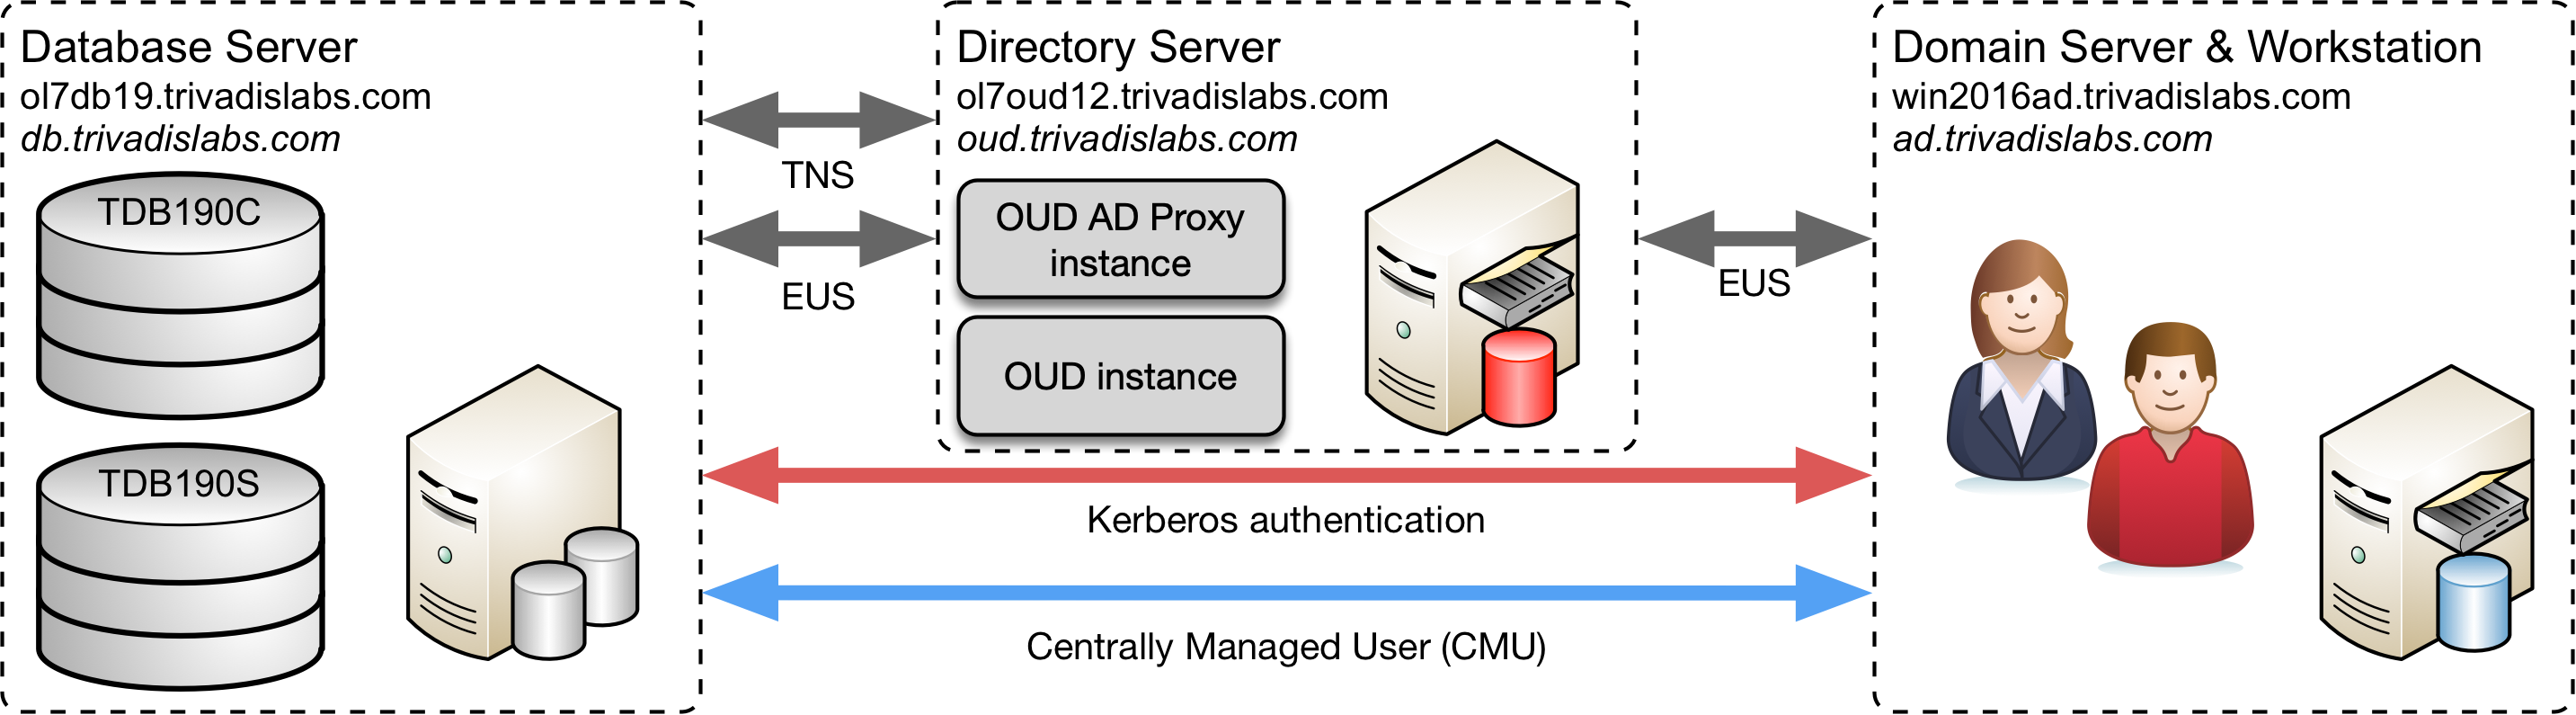
\includegraphics{examples/images/LabEnvironment.png} \emph{Abb. 2:
Architektur Schulungsumgebung}

\hypertarget{uxfcbung-01-titel-der-uxfcbung}{%
\subsection{Übung 01: Titel der
Übung}\label{uxfcbung-01-titel-der-uxfcbung}}

\hypertarget{uxfcbungsziel}{%
\subsubsection{Übungsziel}\label{uxfcbungsziel}}

Etwas lernen\ldots{}

\hypertarget{aufgabe}{%
\subsubsection{Aufgabe}\label{aufgabe}}

\begin{itemize}
\tightlist
\item
  Erstellen HTTP Servers für das Software Repository basierend auf dem
  Images \passthrough{\lstinline!busybox!}.
\item
  Erstellen einer \passthrough{\lstinline!docker-compose!} Datei für das
  automatische starten des HTTP Servers.
\item
  Einbinden der Software via Volume.
\item
  Sicherstellen des Zugriffs auf das HTTP Server.
\end{itemize}

Zusatzaufgabe und weitere Überlegungen:

\begin{itemize}
\tightlist
\item
  Wieso wird gerade \passthrough{\lstinline!busybox!} als basis für
  diesen HTTP Server verwendet?
\item
  Welche weiteren Basis-Images lassen sich ebenfalls verwenden?
\item
  Wozu dient diese Software Repository?
\item
  Was für Alternative zum Download der Software beim Build der Docker
  Images gibt es?
\end{itemize}

\textbf{Vorsausetzungen:} Für diese Übung müssen die folgenden
Anforderungen erfüllt sein:

\begin{itemize}
\tightlist
\item
  Sicherstellen des Zugriffs auf die Docker Übungs- und
  Entwicklungsumgebung
\end{itemize}

\hypertarget{luxf6sung-01-titel-der-uxfcbung}{%
\subsection{Lösung 01: Titel der
Übung}\label{luxf6sung-01-titel-der-uxfcbung}}

Für diese Übung werden folgende Punkte umgesetzt:

\begin{itemize}
\tightlist
\item
  Interaktives starten eines Docker Containers mit
  \passthrough{\lstinline!docker run!}
\item
  Erstellen einer \passthrough{\lstinline!docker-compose!} Datei.
\end{itemize}

\hypertarget{detaillierte-luxf6sungsschritte}{%
\subsubsection{Detaillierte
Lösungsschritte}\label{detaillierte-luxf6sungsschritte}}

Es muss folgendes gemacht werden

\begin{itemize}
\tightlist
\item
  Sicherstellen des Zugriffs auf die Docker Übungs- und
  Entwicklungsumgebung
\end{itemize}

\hypertarget{uxfcbung-02-titel-der-uxfcbung}{%
\subsection{Übung 02: Titel der
Übung}\label{uxfcbung-02-titel-der-uxfcbung}}

\hypertarget{uxfcbungsziel-1}{%
\subsubsection{Übungsziel}\label{uxfcbungsziel-1}}

Etwas lernen\ldots{}

\hypertarget{aufgabe-1}{%
\subsubsection{Aufgabe}\label{aufgabe-1}}

\begin{itemize}
\tightlist
\item
  Erstellen HTTP Servers für das Software Repository basierend auf dem
  Images \passthrough{\lstinline!busybox!}.
\item
  Erstellen einer \passthrough{\lstinline!docker-compose!} Datei für das
  automatische starten des HTTP Servers.
\item
  Einbinden der Software via Volume.
\item
  Sicherstellen des Zugriffs auf das HTTP Server.
\end{itemize}

Zusatzaufgabe und weitere Überlegungen:

\begin{itemize}
\tightlist
\item
  Wieso wird gerade \passthrough{\lstinline!busybox!} als basis für
  diesen HTTP Server verwendet?
\item
  Welche weiteren Basis-Images lassen sich ebenfalls verwenden?
\item
  Wozu dient diese Software Repository?
\item
  Was für Alternative zum Download der Software beim Build der Docker
  Images gibt es?
\end{itemize}

\textbf{Vorsausetzungen:} Für diese Übung müssen die folgenden
Anforderungen erfüllt sein:

\begin{itemize}
\tightlist
\item
  Sicherstellen des Zugriffs auf die Docker Übungs- und
  Entwicklungsumgebung
\end{itemize}

\hypertarget{luxf6sung-02-titel-der-uxfcbung}{%
\subsection{Lösung 02: Titel der
Übung}\label{luxf6sung-02-titel-der-uxfcbung}}

Für diese Übung werden folgende Punkte umgesetzt:

\begin{itemize}
\tightlist
\item
  Interaktives starten eines Docker Containers mit
  \passthrough{\lstinline!docker run!}
\item
  Erstellen einer \passthrough{\lstinline!docker-compose!} Datei.
\end{itemize}

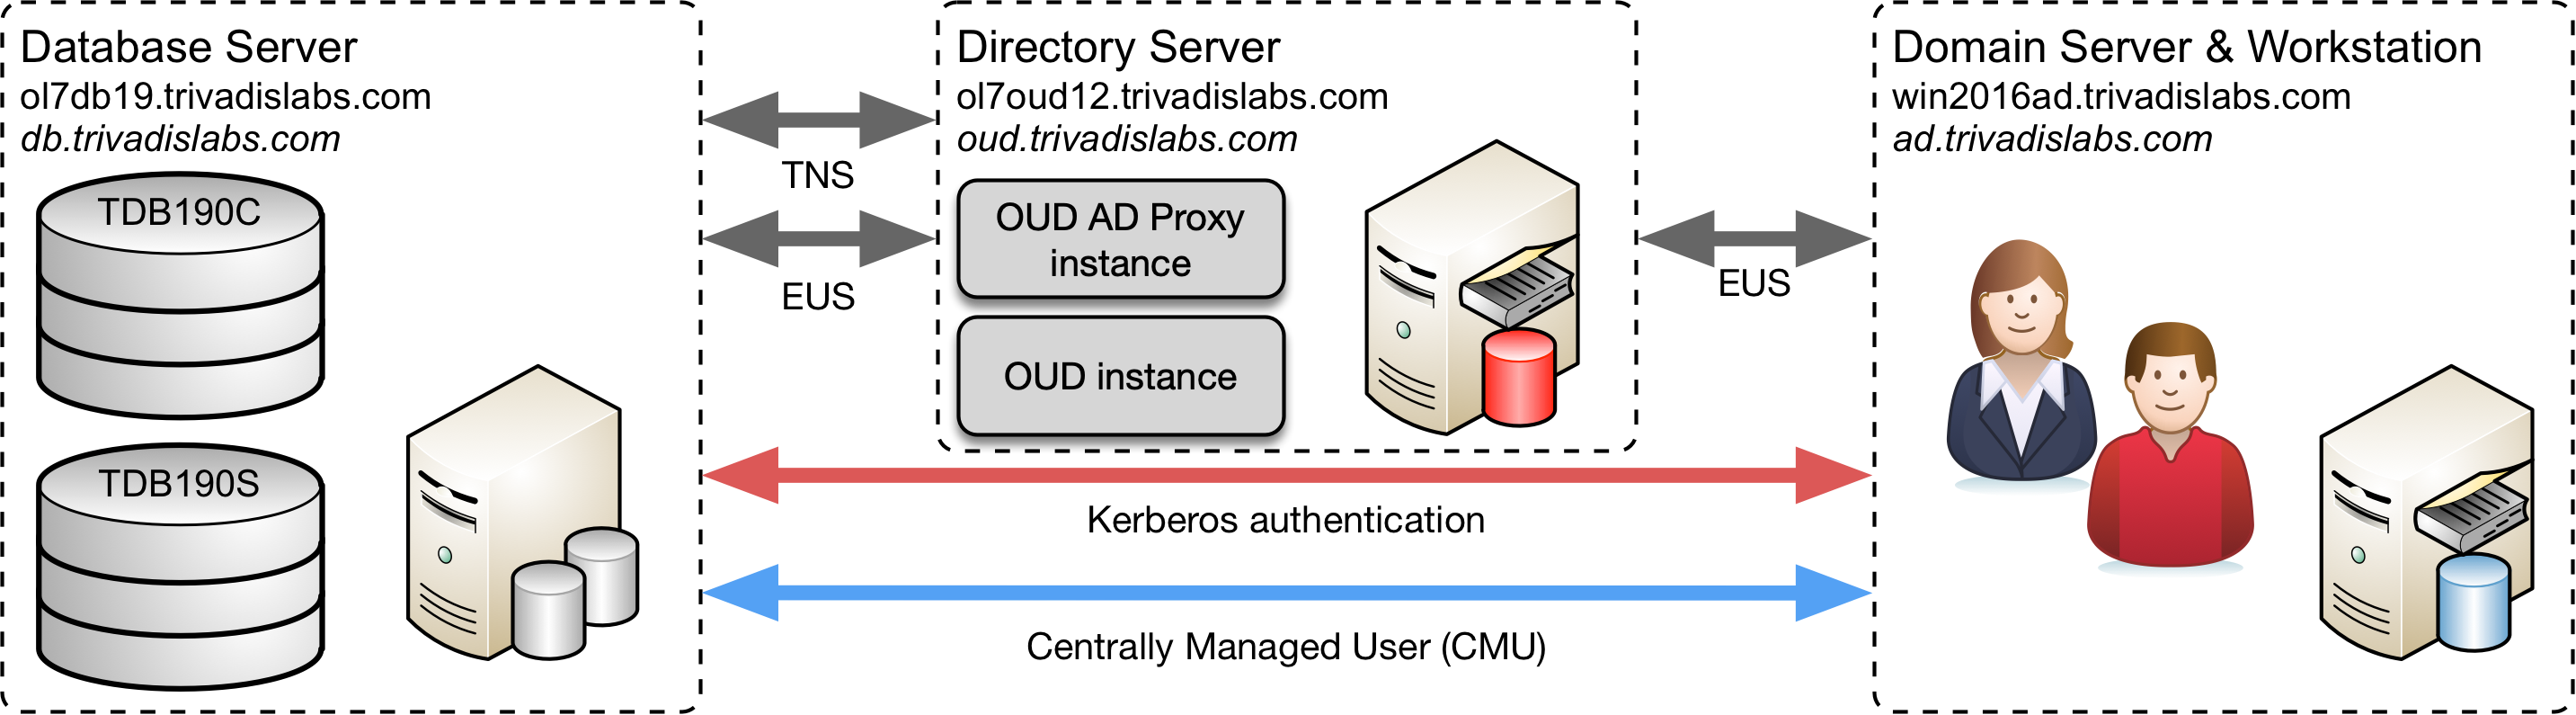
\includegraphics{examples/images/LabEnvironment.png} \emph{Abb. 2:
Architektur Schulungsumgebung}

\hypertarget{detaillierte-luxf6sungsschritte-1}{%
\subsubsection{Detaillierte
Lösungsschritte}\label{detaillierte-luxf6sungsschritte-1}}

Es muss folgendes gemacht werden

\begin{itemize}
\tightlist
\item
  Sicherstellen des Zugriffs auf die Docker Übungs- und
  Entwicklungsumgebung
\end{itemize}

\hypertarget{anhang-b-quellen}{%
\section{Anhang B: Quellen}\label{anhang-b-quellen}}

Die folgenden Verweise sind im Zusammenhang mit dem Trivadis CPU Report
nützlich und haben bei der Erstellung dieses Berichts geholfen.

Allgemeine Informationen zur Oracle Critical Patch Advisory:

\begin{itemize}
\tightlist
\item
  Oracle Recommended Patches Oracle JavaVM Component Database PSU (OJVM
  PSU) Patches
  (\href{https://support.oracle.com/epmos/faces/DocumentDisplay?id=1929745.1}{1929745.1})
\item
  Patch Set Updates Known Issues Notes
  (\href{https://support.oracle.com/epmos/faces/DocumentDisplay?id=1227443.1}{1227443.1})
\item
  Database Security Patching from 12.1.0.1 onwards
  (\href{https://support.oracle.com/epmos/faces/DocumentDisplay?id=1581950.1}{1581950.1})
\item
  Quick Reference to Patch Numbers for Database PSU, SPU(CPU), Bundle
  Patches and Patchsets
  (\href{https://support.oracle.com/epmos/faces/DocumentDisplay?id=1454618.1}{1454618.1})
\item
  Risk Matrix Glossary -- terms and definitions for Critical Patch
  Update risk matrices
  (\href{https://support.oracle.com/epmos/faces/DocumentDisplay?id=394486.1}{394486.1})
\item
  Use of Common Vulnerability Scoring System (CVSS) by Oracle
  (\href{https://support.oracle.com/epmos/faces/DocumentDisplay?id=394487.1}{394487.1})
\item
  Release Schedule of Current Database Releases
  (\href{https://support.oracle.com/epmos/faces/DocumentDisplay?id=742060.1}{742060.1})
\end{itemize}

Informationen über das aktuelle Critical Patch Update:

\begin{itemize}
\tightlist
\item
  Official Oracle web site for this patch
  \href{https://www.oracle.com/technetwork/security-advisory/cpuoct2019-5072832.html}{Oracle
  Critical Patch Update Advisory - October 2019}
\item
  Text Form of Oracle Critical Patch Update -
  \href{https://www.oracle.com/technetwork/security-advisory/cpuoct2019verbose-5072833.html}{October
  2019 Risk Matrices}
\item
  Oracle Critical Patch Update October 2019 Documentation Map - MOS Note
  \href{https://support.oracle.com/epmos/faces/DocumentDisplay?id=2566013.1}{2566013.1}
\item
  Critical Patch Update (CPU) Program Oct 2019 Patch Availability
  Document (PAD)
  \href{https://support.oracle.com/epmos/faces/DocumentDisplay?id=2568292.1}{2568292.1}
\item
  Oracle Database / Grid Infrastructure / OJVM Release Update \& Release
  Update Revision 12.2.0.1 Jul 2018 Known Issues - MOS Note
  \href{https://support.oracle.com/epmos/faces/DocumentDisplay?id=2359048.1}{2359048.1}
\item
  Known Issues for Oracle WebLogic Server (OWLS) 12.1.3.0.X Patch Set
  Updates - MOS Note
  \href{https://support.oracle.com/epmos/faces/DocumentDisplay?id=2137518.1}{2137518.1}
\item
  Known Issues for Oracle WebLogic Server (OWLS) 12.2.1.3.X Patch Set
  Updates - MOS Note
  \href{https://support.oracle.com/epmos/faces/DocumentDisplay?id=2350415.1}{2350415.1}
\item
  12.1.0.2 Patch Set - Availability and Known Issues - MOS Note
  \href{https://support.oracle.com/epmos/faces/DocumentDisplay?id=1683799.1}{1683799.1}
\item
  12.2.0.1 Base Release - Availability and Known Issues - MOS Note
  \href{https://support.oracle.com/epmos/faces/DocumentDisplay?id=2239820.1}{2239820.1}
\item
  18.0.0.0 Base Release - Availability and Known Issues - MOS Note
  \href{https://support.oracle.com/epmos/faces/DocumentDisplay?id=2387295.1}{2387295.1}
\end{itemize}

Datenbanksicherheitsstandards und Best Practice:

\begin{itemize}
\tightlist
\item
  CIS Oracle Database Benchmarks -
  \url{https://www.cisecurity.org/benchmark/oracle_database/}
\item
  STIGs Document Library -
  \href{https://public.cyber.mil/stigs/downloads/?_dl_facet_stigs=app-security\%2Cdatabase}{Database
  STIG}
\item
  Common Vulnerability Scoring System
  \href{http://www.first.org/cvss/}{CVSS}
\end{itemize}

\hypertarget{appendix-a-glossary}{%
\section{Appendix A: Glossary}\label{appendix-a-glossary}}

\begin{itemize}
\tightlist
\item
  \textbf{API} -- Application programming interface
\item
  \textbf{BSU} - BEA Smart Update ist ein Dienstprogramm, um Patches auf
  WebLogic Server einzuspielen
\item
  \textbf{CA} -- Certificate Authority
\item
  \textbf{CLI} -- Command Line Interface
\item
  \textbf{CPU} - Critical Patch Update
\item
  \textbf{CVSS} - Common Vulnerability Scoring System
  \href{http://www.first.org/cvss}{CVSS}
\item
  \textbf{EUS} - Oracle Enterprise User Security
\item
  \textbf{IAM} - Identity and Access Management
\item
  \textbf{LDAP} -- Lightweight Directory Access Protocol
\item
  \textbf{OUD} - Oracle Unified Directory
\item
  \textbf{PSU} - Patch Set Update
\item
  \textbf{RBAC} -- Role-Based Access Control
\item
  \textbf{RDP} -- Remote Desktop Protocol
\item
  \textbf{RU} - Release Update
\item
  \textbf{SPU} - Security Patch Update
\item
  \textbf{SSH} -- Secure Shell
\item
  \textbf{SSL} -- Secure Sockets Layer
\item
  \textbf{SSO} -- Single Sign-On
\item
  \textbf{TLS} -- Transport Layer Security, the successor to Secure
  Sockets Layer (SSL)
\end{itemize}
